\clearpage

\section{Sample mock data fits}

In order for the reader to gain an understanding of the difficulties involved in fitting the reconstructed
energy spectrum from a $3.23 \times 10^{19}$ POT dataset
(just over 6 1-ring $\mu$-like events are expected by both GENIE and NEUT for oscillations with
$sin^{2}2\theta_{23}$ = 1.00 and $\Delta m^{2}_{23}$ = 2.4$\times10^{-3}$ $eV^{2}/c^{4}$),
we present a series of mock-dataset fits (Figs. \ref{fig:mock_data_fit_1} - \ref{fig:mock_data_fit_8}).
The mock-dataset were both generated 
(with true oscillation parameters $sin^{2}2\theta_{23}$ = 1.00 and $\Delta m^{2}_{23}$ = 2.4$\times10^{-3}$ $eV^{2}/c^{4}$)
and fitted using the GENIE p.d.f's.
In each figure, the top-left plot shows the reconstructed energies of the mock-dataset and the best-fit prediction.
The confidence regions shown on the top-right are the 68\% and 90\% CL regions (statistical errors only) 
calculated using the PDG method 
(Sec. \ref{sec:contour_pdg}).
For reference, the MINOS 90\% CL region is also shown (red line).
The best-fit point is shown with a black-star while the input point is indicated by a red circle.
The bottom-left and bottom-right plots show the $\chi^{2}$/ndof along the  $sin^{2}2\theta_{23}$ and $\Delta m^{2}_{23}$
lines that pass through the best-fit point\footnote{
 Note that they {\em are not} marginalized $\chi^{2}$/ndof distributions as functions of $sin^{2}2\theta_{23}$ and $\Delta m^{2}_{23}$.
}.
Finally, in Fig. \ref{fig:mock_data_fits_summary} we show the best-fit point distribution from a set of 5,000 mock-dataset fits.

\begin{figure}[htb]
\center
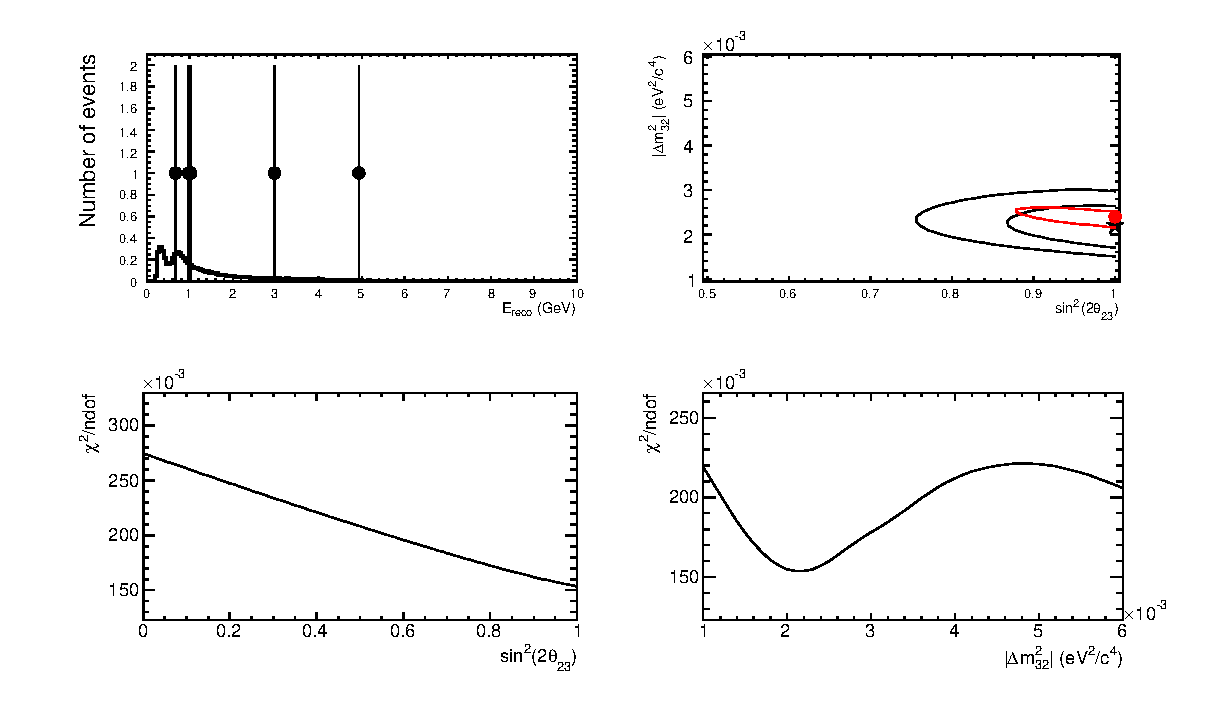
\includegraphics[height=22pc]{./images/fits/mock_sample/mock_fit_1.eps}
\caption{
  Mock-dataset fit 1:
  The reconstructed neutrino energies of the mock 1-ring $\mu$-like data sample
  are \{0.652999, 0.972174, 1.0032, 2.98126, 4.91308\} GeV.
  The best-fit oscillation parameters are 
  $sin^{2}2\theta_{23}$ = 1.00 and $\Delta m^{2}_{23}$ = 2.2$\times10^{-3}$ $eV^{2}/c^{4}$.
}
\label{fig:mock_data_fit_1}
\end{figure}

\begin{figure}[htb]
\center
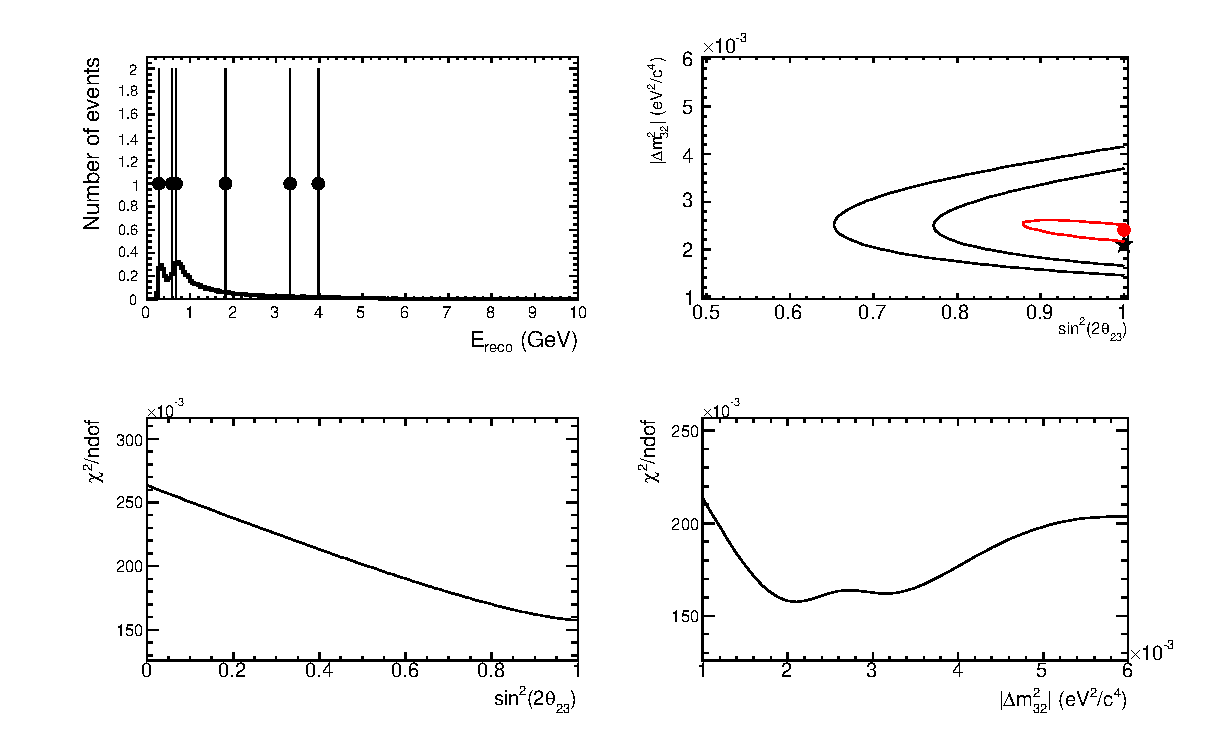
\includegraphics[height=20pc]{./images/fits/mock_sample/mock_fit_2.eps}
\caption{
  Mock-dataset fit 2:
  The reconstructed neutrino energies of the mock 1-ring $\mu$-like data sample
  are \{0.253796, 0.574917, 0.654082, 1.82992, 3.33207, 3.95891\} GeV.
  The best-fit oscillation parameters are 
  $sin^{2}2\theta_{23}$ = 1.00 and $\Delta m^{2}_{23}$ = 2.1$\times10^{-3}$ $eV^{2}/c^{4}$.
}
\label{fig:mock_data_fit_2}
\end{figure}

\begin{figure}[htb]
\center
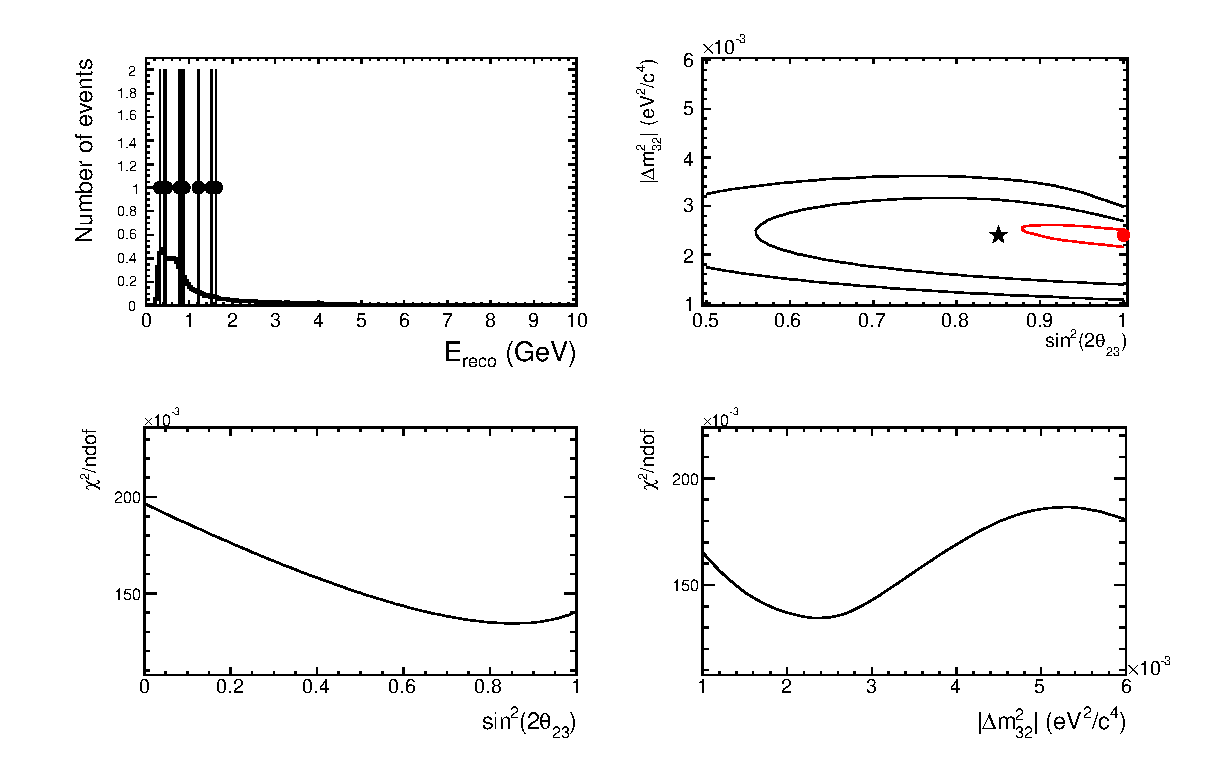
\includegraphics[height=20pc]{./images/fits/mock_sample/mock_fit_3.eps}
\caption{
  Mock-dataset fit 3:
  The reconstructed neutrino energies of the mock 1-ring $\mu$-like data sample
  are \{0.32655, 0.427434, 0.480255, 0.774868, 0.841949, 0.85971, 1.24938, 1.5061, 1.63616\} GeV.
  The best-fit oscillation parameters are 
  $sin^{2}2\theta_{23}$ = 0.85 and $\Delta m^{2}_{23}$ = 2.4$\times10^{-3}$ $eV^{2}/c^{4}$.
}
\label{fig:mock_data_fit_3}
\end{figure}

\begin{figure}[htb]
\center
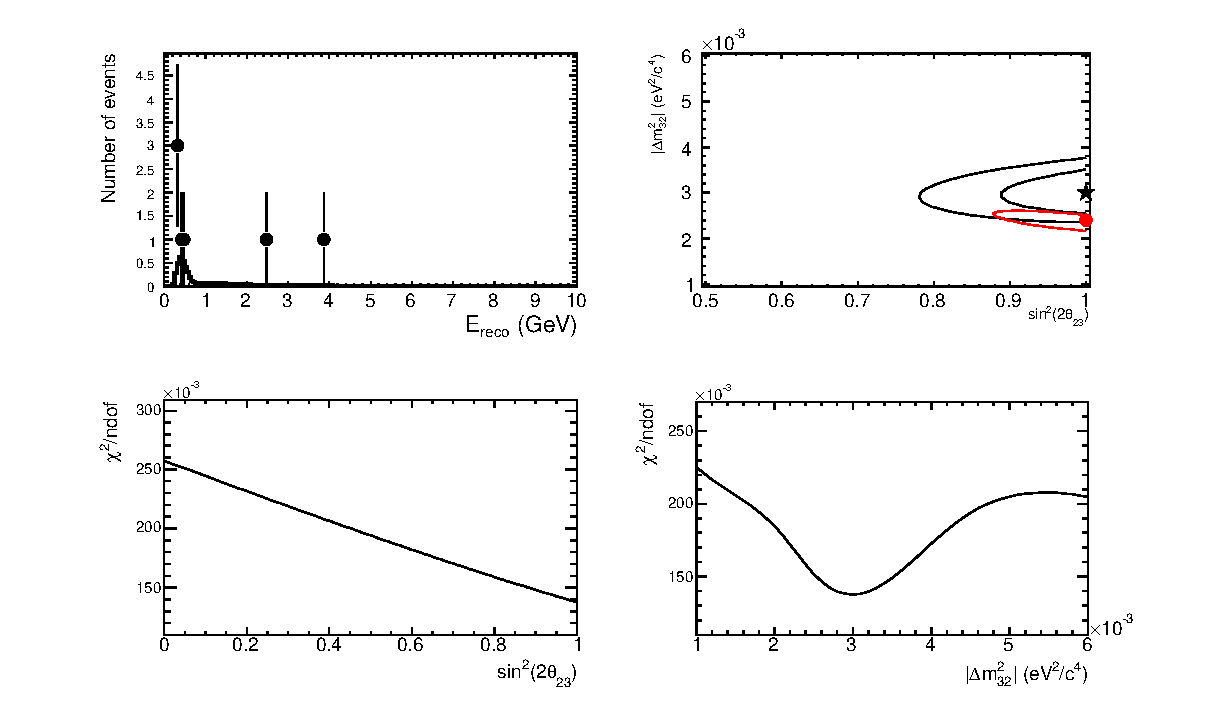
\includegraphics[height=20pc]{./images/fits/mock_sample/mock_fit_4.eps}
\caption{
  Mock-dataset fit 4:
  The reconstructed neutrino energies of the mock 1-ring $\mu$-like data sample
  are \{0.310258, 0.343666, 0.346476, 0.429402, 0.455564, 2.48224, 3.87468\} GeV.
  The best-fit oscillation parameters are 
  $sin^{2}2\theta_{23}$ = 1.00 and $\Delta m^{2}_{23}$ = 3.0$\times10^{-3}$ $eV^{2}/c^{4}$.
}
\label{fig:mock_data_fit_4}
\end{figure}

\begin{figure}[htb]
\center
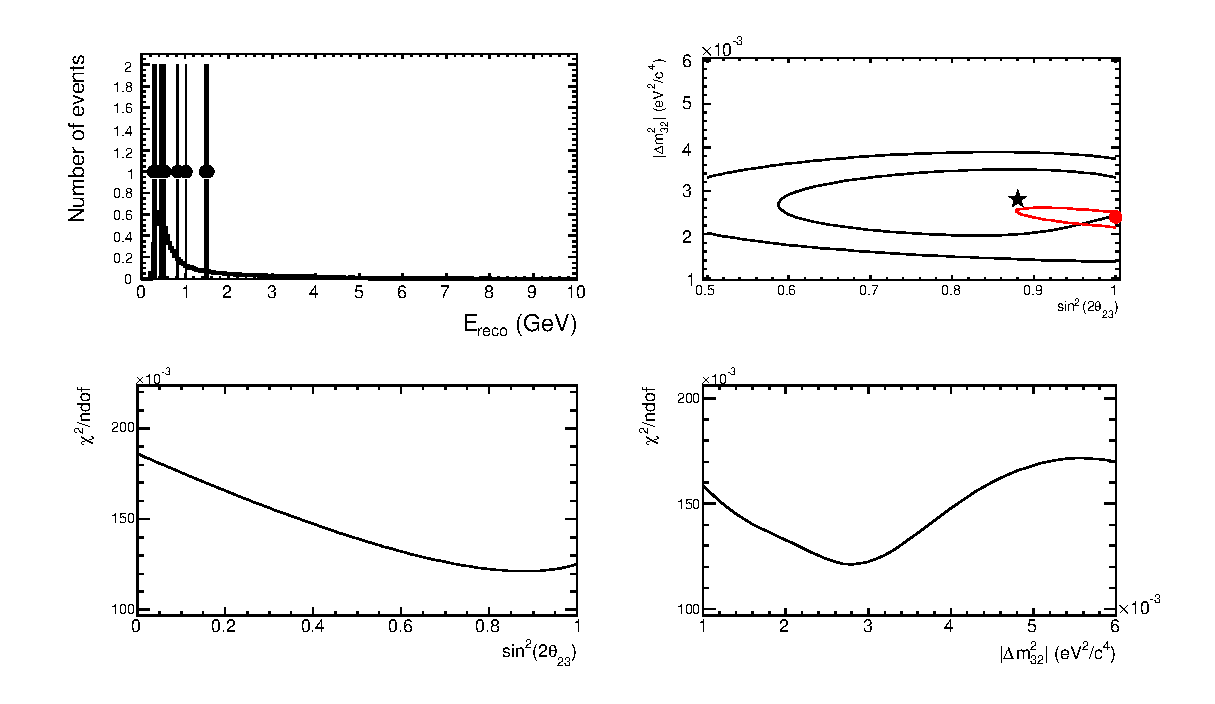
\includegraphics[height=20pc]{./images/fits/mock_sample/mock_fit_5.eps}
\caption{
  Mock-dataset fit 5:
  The reconstructed neutrino energies of the mock 1-ring $\mu$-like data sample
  are \{0.28082, 0.328775, 0.44747, 0.45361, 0.543383, 0.812863, 1.03911, 1.45479, 1.53207\} GeV.
  The best-fit oscillation parameters are 
  $sin^{2}2\theta_{23}$ = 0.88 and $\Delta m^{2}_{23}$ = 2.8$\times10^{-3}$ $eV^{2}/c^{4}$.
}
\label{fig:mock_data_fit_5}
\end{figure}

\begin{figure}[htb]
\center
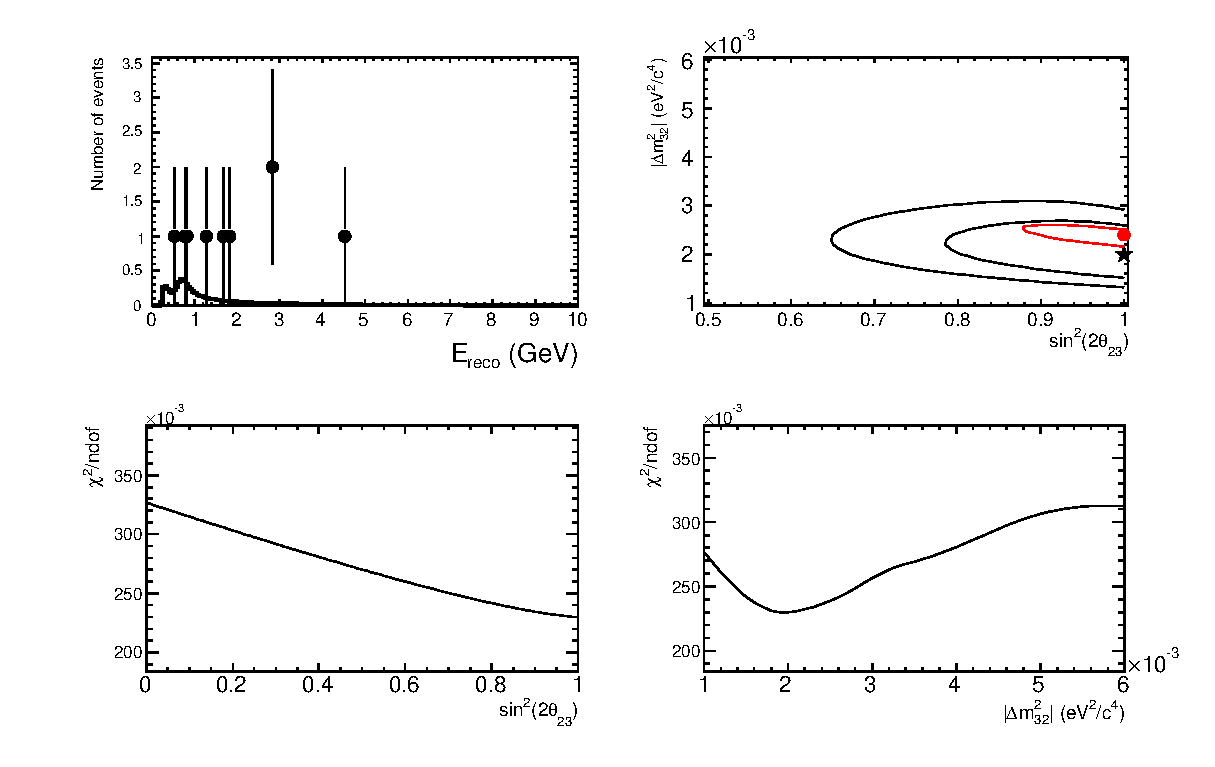
\includegraphics[height=20pc]{./images/fits/mock_sample/mock_fit_6.eps}
\caption{
  Mock-dataset fit 6:
  The reconstructed neutrino energies of the mock 1-ring $\mu$-like data sample
  are \{0.540056, 0.771411, 0.815833, 1.27384, 1.69788, 1.8422, 2.84393, 2.8057, 4.5466\} GeV.
  The best-fit oscillation parameters are 
  $sin^{2}2\theta_{23}$ = 1.00 and $\Delta m^{2}_{23}$ = 2.0$\times10^{-3}$ $eV^{2}/c^{4}$.
}
\label{fig:mock_data_fit_6}
\end{figure}

\begin{figure}[htb]
\center
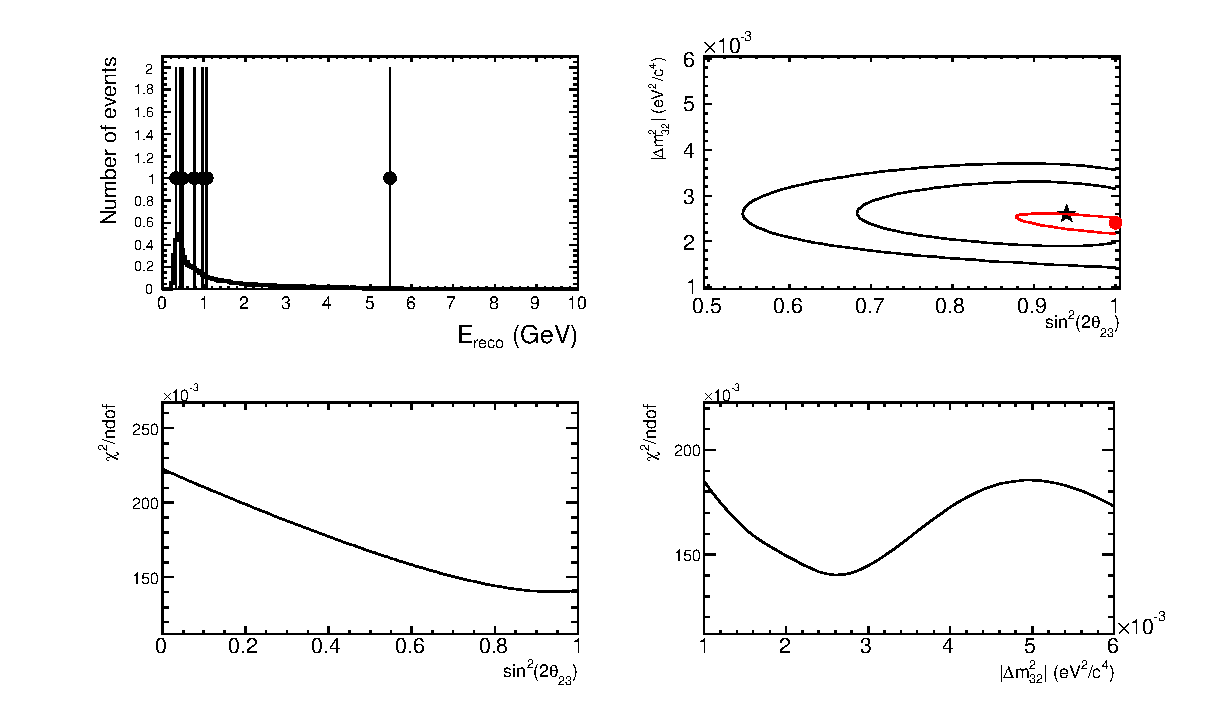
\includegraphics[height=20pc]{./images/fits/mock_sample/mock_fit_7.eps}
\caption{
  Mock-dataset fit 7:
  The reconstructed neutrino energies of the mock 1-ring $\mu$-like data sample
  are \{0.319674, 0.407844, 0.462414, 0.759538, 0.968712, 1.06938, 5.4639\} GeV.
  The best-fit oscillation parameters are 
  $sin^{2}2\theta_{23}$ = 0.94 and $\Delta m^{2}_{23}$ = 2.6$\times10^{-3}$ $eV^{2}/c^{4}$.
}
\label{fig:mock_data_fit_7}
\end{figure}

\begin{figure}[htb]
\center
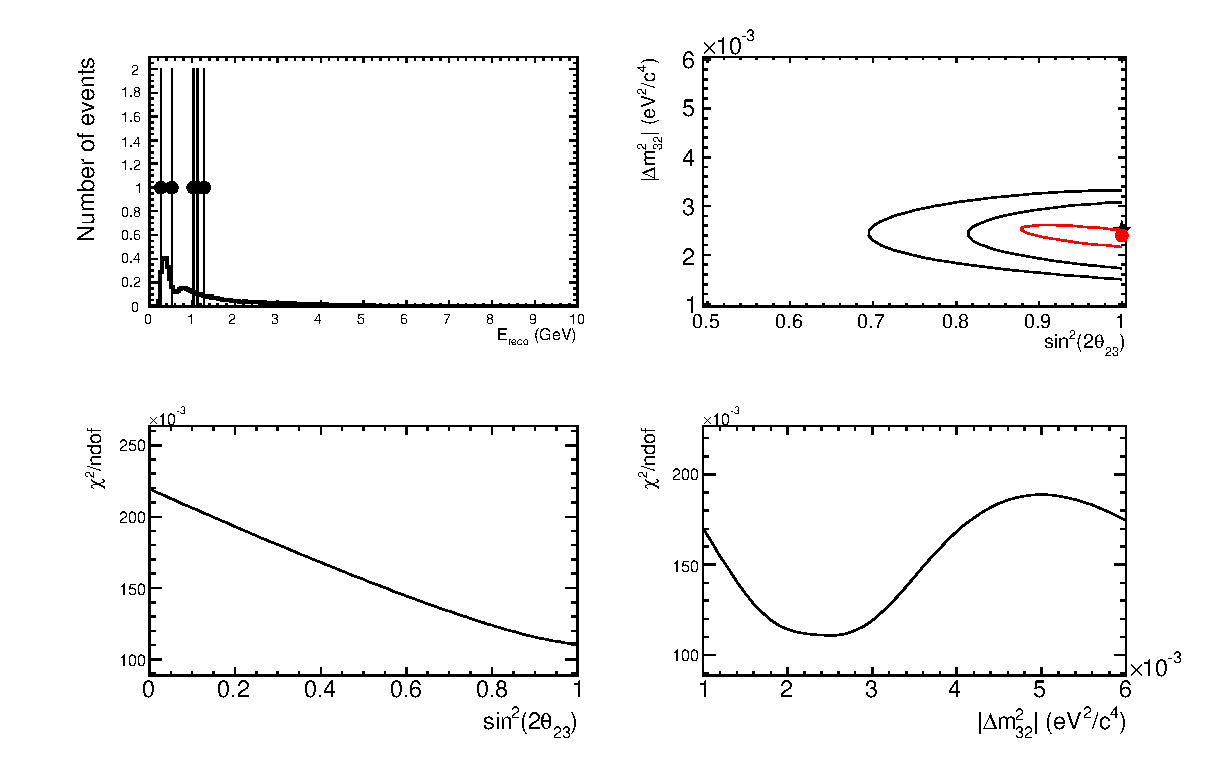
\includegraphics[height=20pc]{./images/fits/mock_sample/mock_fit_8.eps}
\caption{
  Mock-dataset fit 8:
  The reconstructed neutrino energies of the mock 1-ring $\mu$-like data sample
  are \{0.264395, 0.530563, 1.01775, 1.12194, 1.28155\} GeV.
  The best-fit oscillation parameters are 
  $sin^{2}2\theta_{23}$ = 1.00 and $\Delta m^{2}_{23}$ = 2.5$\times10^{-3}$ $eV^{2}/c^{4}$.
}
\label{fig:mock_data_fit_8}
\end{figure}

\begin{figure}[htb]
\center
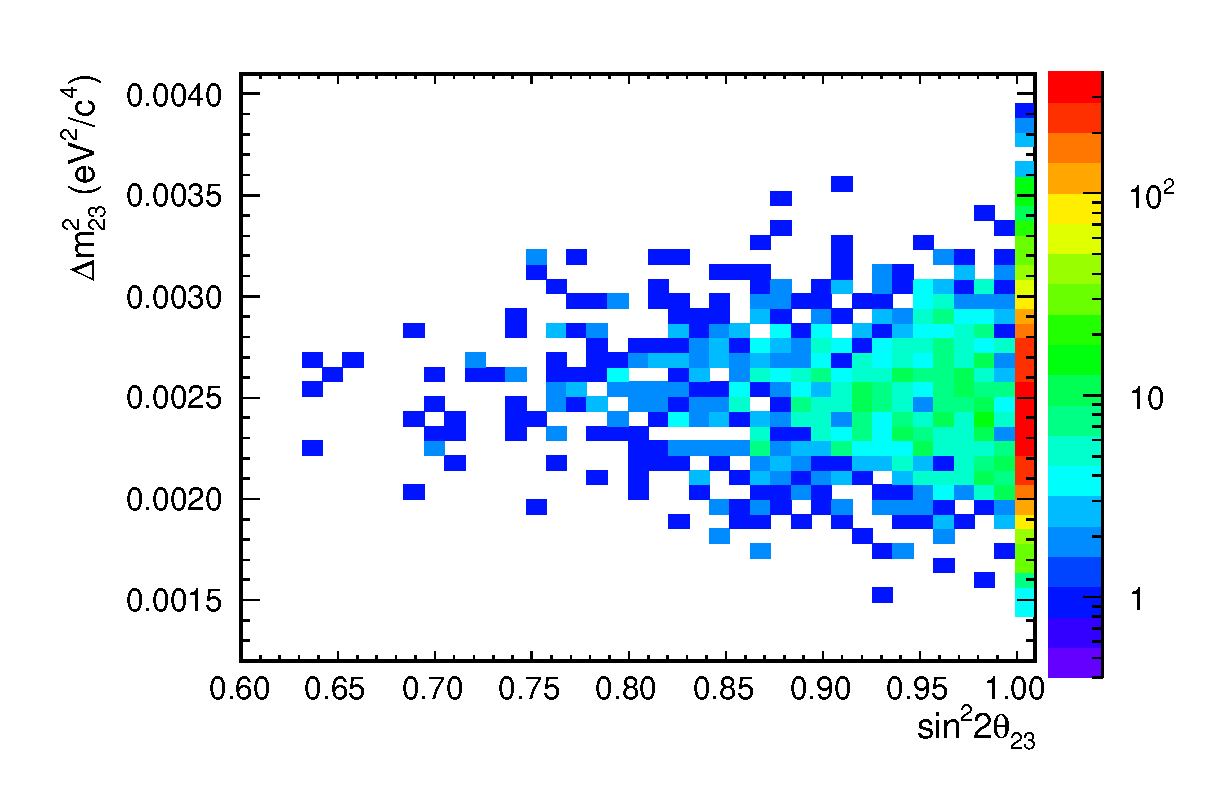
\includegraphics[height=20pc]{./images/fits/mock_sample/bestpoints_5k_mockfits.eps}
\caption{
  Distribution of best-fit oscillation parameters for 5,000 mock-dataset fits.
}
\label{fig:mock_data_fits_summary}
\end{figure}
